\section{Experimental Settings}

\subsection{SIMPLER Environment}
The SIMPLER simulation environment serves as our primary benchmark for evaluating VLA models. It is specifically designed to closely mirror real-world robotic setups, thereby facilitating more realistic evaluations and bridging the real-to-sim control and visual gap. 

SIMPLER offers two distinct evaluation settings:
\begin{itemize}
    \item \textbf{Visual Matching (VM):} This setting closely replicates real-world tasks by minimizing discrepancies between the simulated and real environments, prioritizing fidelity to real-world appearances.
    \item \textbf{Variant Aggregation (VA):} This setting builds upon Visual Matching by introducing variations to elements such as background, lighting, distractors, and table texture, challenging models to generalize across diverse conditions.
\end{itemize}



For the Google robot setup, SIMPLER provides both evaluation settings, each featuring the same four tasks: 1) Pick coke can, 2) Move near, 3) Open/close drawer, and 4) Open top drawer and place apple. These four tasks for the Google robot are also illustrated in Figure~\ref{fig:task}.
\begin{figure}[htbp]
    \centering
    % \vspace{-10pt}
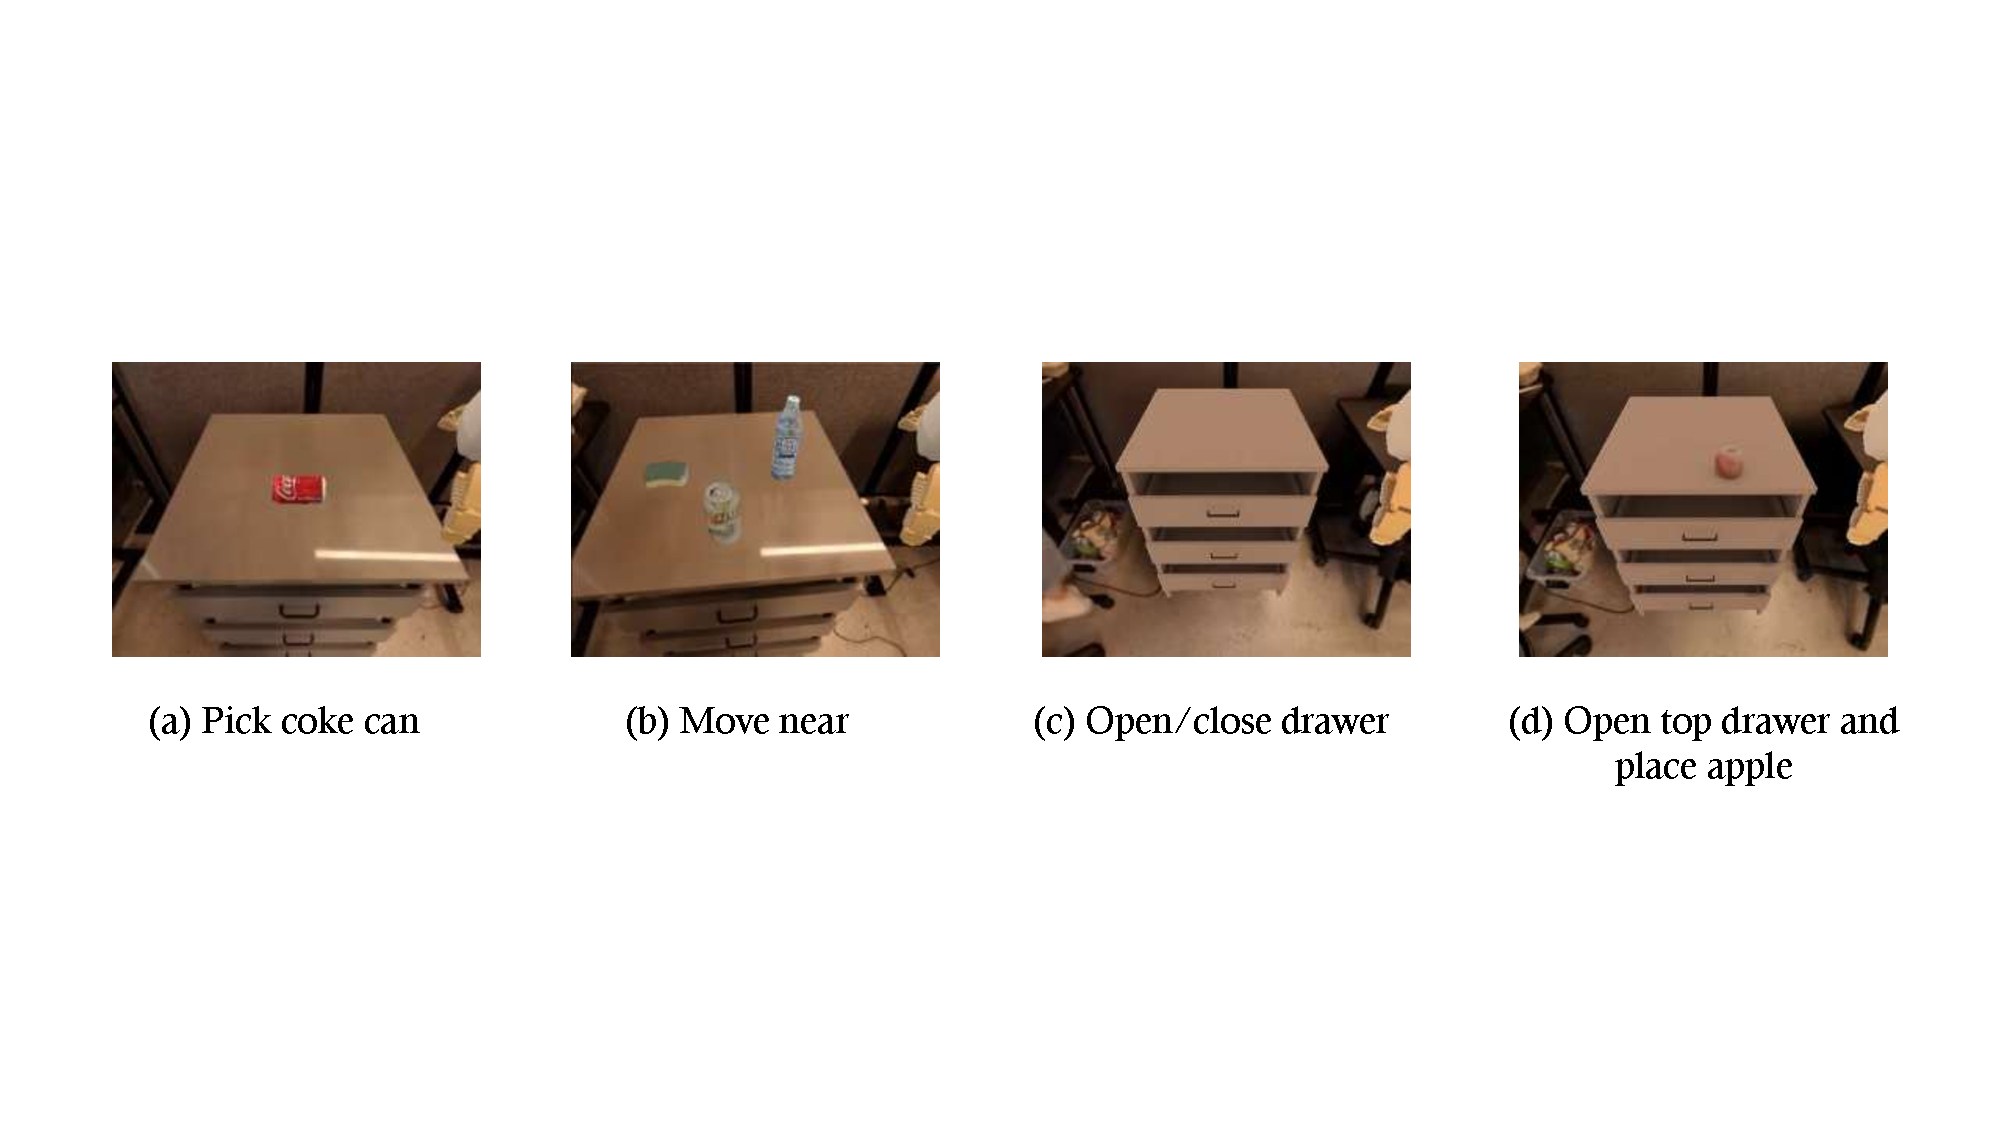
\includegraphics[width=0.99\linewidth]{figs/task.pdf}
    \vspace{-5pt}
    \caption{Representative robotic manipulation tasks for the Google robot in the SIMPLER environment: (a) Pick coke can, (b) Move near, (c) Open/close drawer, and (d) Open top drawer and place apple.}
    \label{fig:task}
    % \vspace{-10pt}
\end{figure}


\subsection{Baselines}
We benchmark our EfficientVLA against the following relevant baseline and backbone methodologies:
\begin{itemize}
    \item \textbf{CogACT:} This model serves as our primary experimental validation platform. CogACT integrates powerful vision encoders (DINOv2 and SigLIP) to process raw visual input, a Llama2-7B language module for multimodal reasoning, and a Diffusion Transformer (DiT) as a specialized action module for generating precise action trajectories. It aims to synergize "cognition" (VLM output) with "action" capabilities by conditioning the diffusion-based action module on the VLM's extracted features, addressing the continuous, multimodal, and temporally correlated nature of robot actions.

    \item \textbf{VLA-Cache:} This is a training-free acceleration method designed to improve VLA model efficiency in robotic manipulation. VLA-Cache operates on the principle that visual inputs in sequential robotic tasks often exhibit minimal variation between successive steps, particularly in background regions. It incorporates a token-selection mechanism that identifies visually static tokens with minimal changes from the previous step and reuses their computational results via KV-cache. Additionally, it includes a fine-grained selection scheme to filter out critical task-relevant tokens, ensuring they undergo full computation to preserve accuracy, and employs a layer-adaptive strategy to adjust reuse ratios based on attention concentration.

    \item \textbf{FastV:} This approach focuses on accelerating inference in Large Vision-Language Models (LVLMs) by pruning redundant visual tokens. FastV's core insight is the identification of inefficient attention phenomena in deeper layers of popular LVLMs, where image tokens receive significantly less attention despite accounting for a large portion of input tokens. It proposes a plug-and-play method that dynamically prunes a percentage of these less impactful visual tokens after a specific layer, guided by attention scores, to reduce computational costs (FLOPs) without sacrificing performance.
\end{itemize}

\section{Impact Statement}

This paper introduces EfficientVLA, a crucial contribution to Vision-Language-Action (VLA) models by directly addressing their significant computational and memory demands through a novel training-free framework. EfficientVLA synergistically prunes redundant language layers, optimizes visual token selection for task-relevance and diversity, and caches intermediate features in the diffusion-based action head, thereby significantly boosting VLA model efficiency and speed. This enables the practical deployment of powerful VLA models on resource-constrained robotic platforms for real-time interaction, accelerating progress in robotic manipulation and reasoning tasks, and contributing to more development by reducing computational load. We intend this work for ethical academic research and authorized commercial applications and strictly prohibit its use for harmful, unethical, or unlawful robotic actions, underscoring our responsibility to ensure societal benefit aligned with fundamental ethical principles.

\section{Limitations}

While EfficientVLA significantly advances VLA model acceleration, certain limitations warrant discussion. Our training-free approach, may not achieve the maximal compression or speedup attainable by training-aware methods. The fixed cache interval $N$ in the action head introduces a trade-off between acceleration and action fidelity and future work could explore adaptive caching. Furthermore, due to the limited availability of open-source diffusion-based VLA models, our current demonstrations are primarily on CogACT. In the future, we aim to validate scalability and effectiveness of EfficientVLA across a wider range of models and tasks as more such architectures become available.